\section{Begründug zur Ausfilterung bestimmter Fragen aus dem Fragebogen \textcolor{red}{\cite{http://www.uselab.tu-berlin.de/wiki/images/6/62/ISONorm_Kurzversion.pdf}}}

Nachfolgend wird jeweils die positive Ausprägung der gefilterten Fragen aufgelistet.\\

\noindent
Beide Systeme ermöglichen eine einfache Ansicht von Informationen. Die individuelle Arbeitsweise von Personen zur Ansicht/Abarbeitung dieser Informationen, ist kein Bestandteil dieser Untersuchung.
Beide Systeme ermöglichen die benötigte Flexibilität. Daher wurden folgende Fragen aus der Nutzerbefragung entfernt:
\begin{itemize}
    \item Die Software erzwingt keine unnötig starre Einhaltung von Bearbeitungsschritten. (Sk1) % (Sw12)
    \item Die Software erzwingt keine unnötigen Unterbrechungen der Arbeit. (Sk3) % (Sw15)
    \item Die Software lässt sich von mir gut an meine persönliche, individuelle Art der Arbeitserledigung anpassen. (Ik2) % (Sw27)
    \item Die Software lässt sich - im Rahmen ihres Leistungsumfangs - von mir gut für unterschiedliche Aufgaben passend einrichten. (Ik3) % (Sw29)
\end{itemize}

\noindent
Es handelt sich für diesen Use-Case (Testpoolmonitoring) ausschließlich um die Ergebnis-Ansicht als Informationsquelle. Es können keine Eingaben getätigt werden. Interaktionen wie Erweiterung/Veränderung des Dashboards/der Ansicht oder weitere administrative Tätigkeiten, die das Framework Grafana ermöglicht, sind kein Teil der täglichen Aufgabe. Daher wurden folgende Fragen aus der Nutzerbefragung entfernt:
\begin{itemize}
    \item Die Software liefert in zureichendem Maße Informationen darüber, welche Eingaben zulässig oder nötig sind. (sb1) % (Sw08)
    \item Die Software bietet auf Verlangen situationsspezifische Erklärungen, die konkret weiterhelfen. (sb2) % (Sw09)
    \item Die Software informiert in ausreichendem Maße über das, was es gerade macht. (ek2) % (Sw18)
    \item Die Software liefert gut verständliche Fehlermeldungen. (ft1) % (Sw23)
    \item Die Software erfordert bei Fehlern im Großen und Ganzen einen geringen Korrekturaufwand. (ft2) % (Sw24)
    \item Die Software gibt konkrete Hinweise zur Fehlerbehebung. (ft3) % (Sw25)
    \item Die Software lässt sich von mir leicht erweitern, wenn für mich neue Aufgaben entstehen. (Ik1) % (Sw26)
\end{itemize}

\section{gekürzter Fragebogen der Nutzerbefragung nach Prümper}

%Folgende Fragen wurden übernommen: Sw02, Sw04, Sw05, Sw10, Sw13, Sw16, Sw20, Sw31, Sw33 und Sw35. (Reihenfolge abweichend)\textcolor{red}{\cite{https://inf-schule.de/content/9_software/1_gui/1_benutzerfreudlichkeit/3_uebungen/Methode_Isonorm-Fragebogen.pdf}}

Folgende Fragen wurden übernommen: aa1, aa2, aa3, sb3, sk2, ek1, ek3, If1, If2 und If3. (Reihenfolge abweichend) \textcolor{red}{\cite{http://www.uselab.tu-berlin.de/wiki/images/6/62/ISONorm_Kurzversion.pdf}}


\begin{figure} [H]
    \centering
    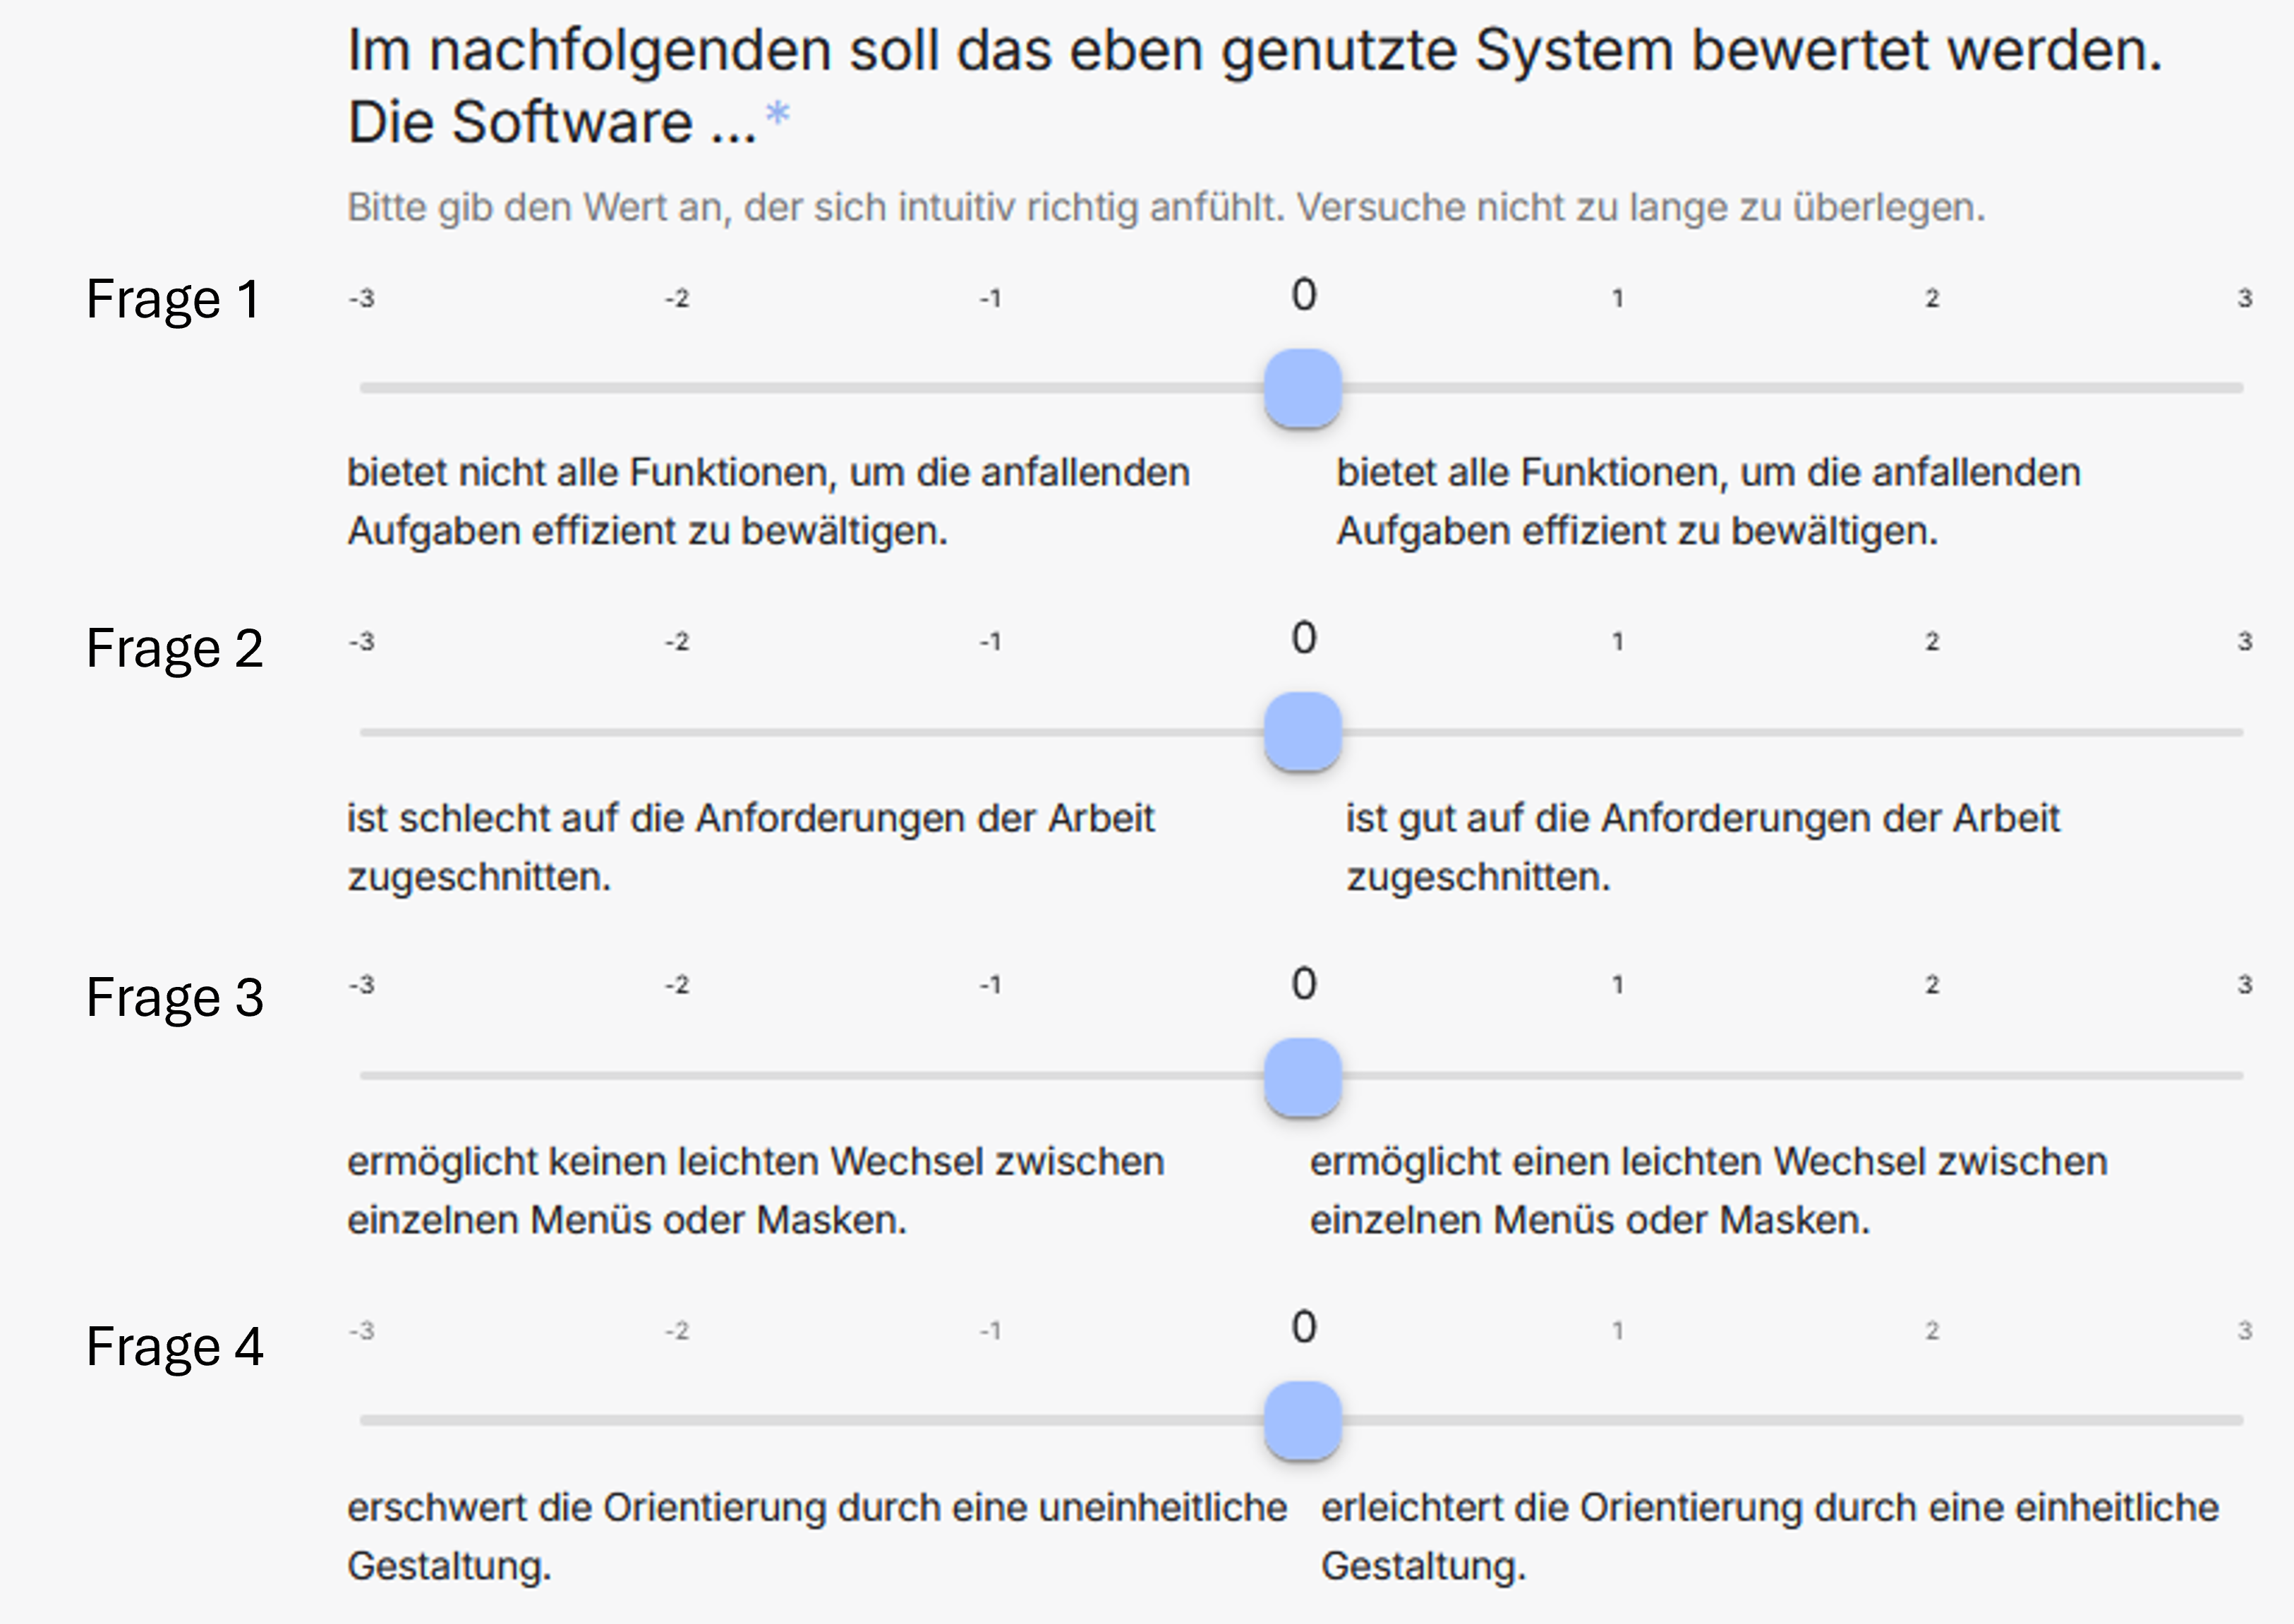
\includegraphics[width=0.85\linewidth]{Anhänge/Survio_Pruemper_1.PNG}
    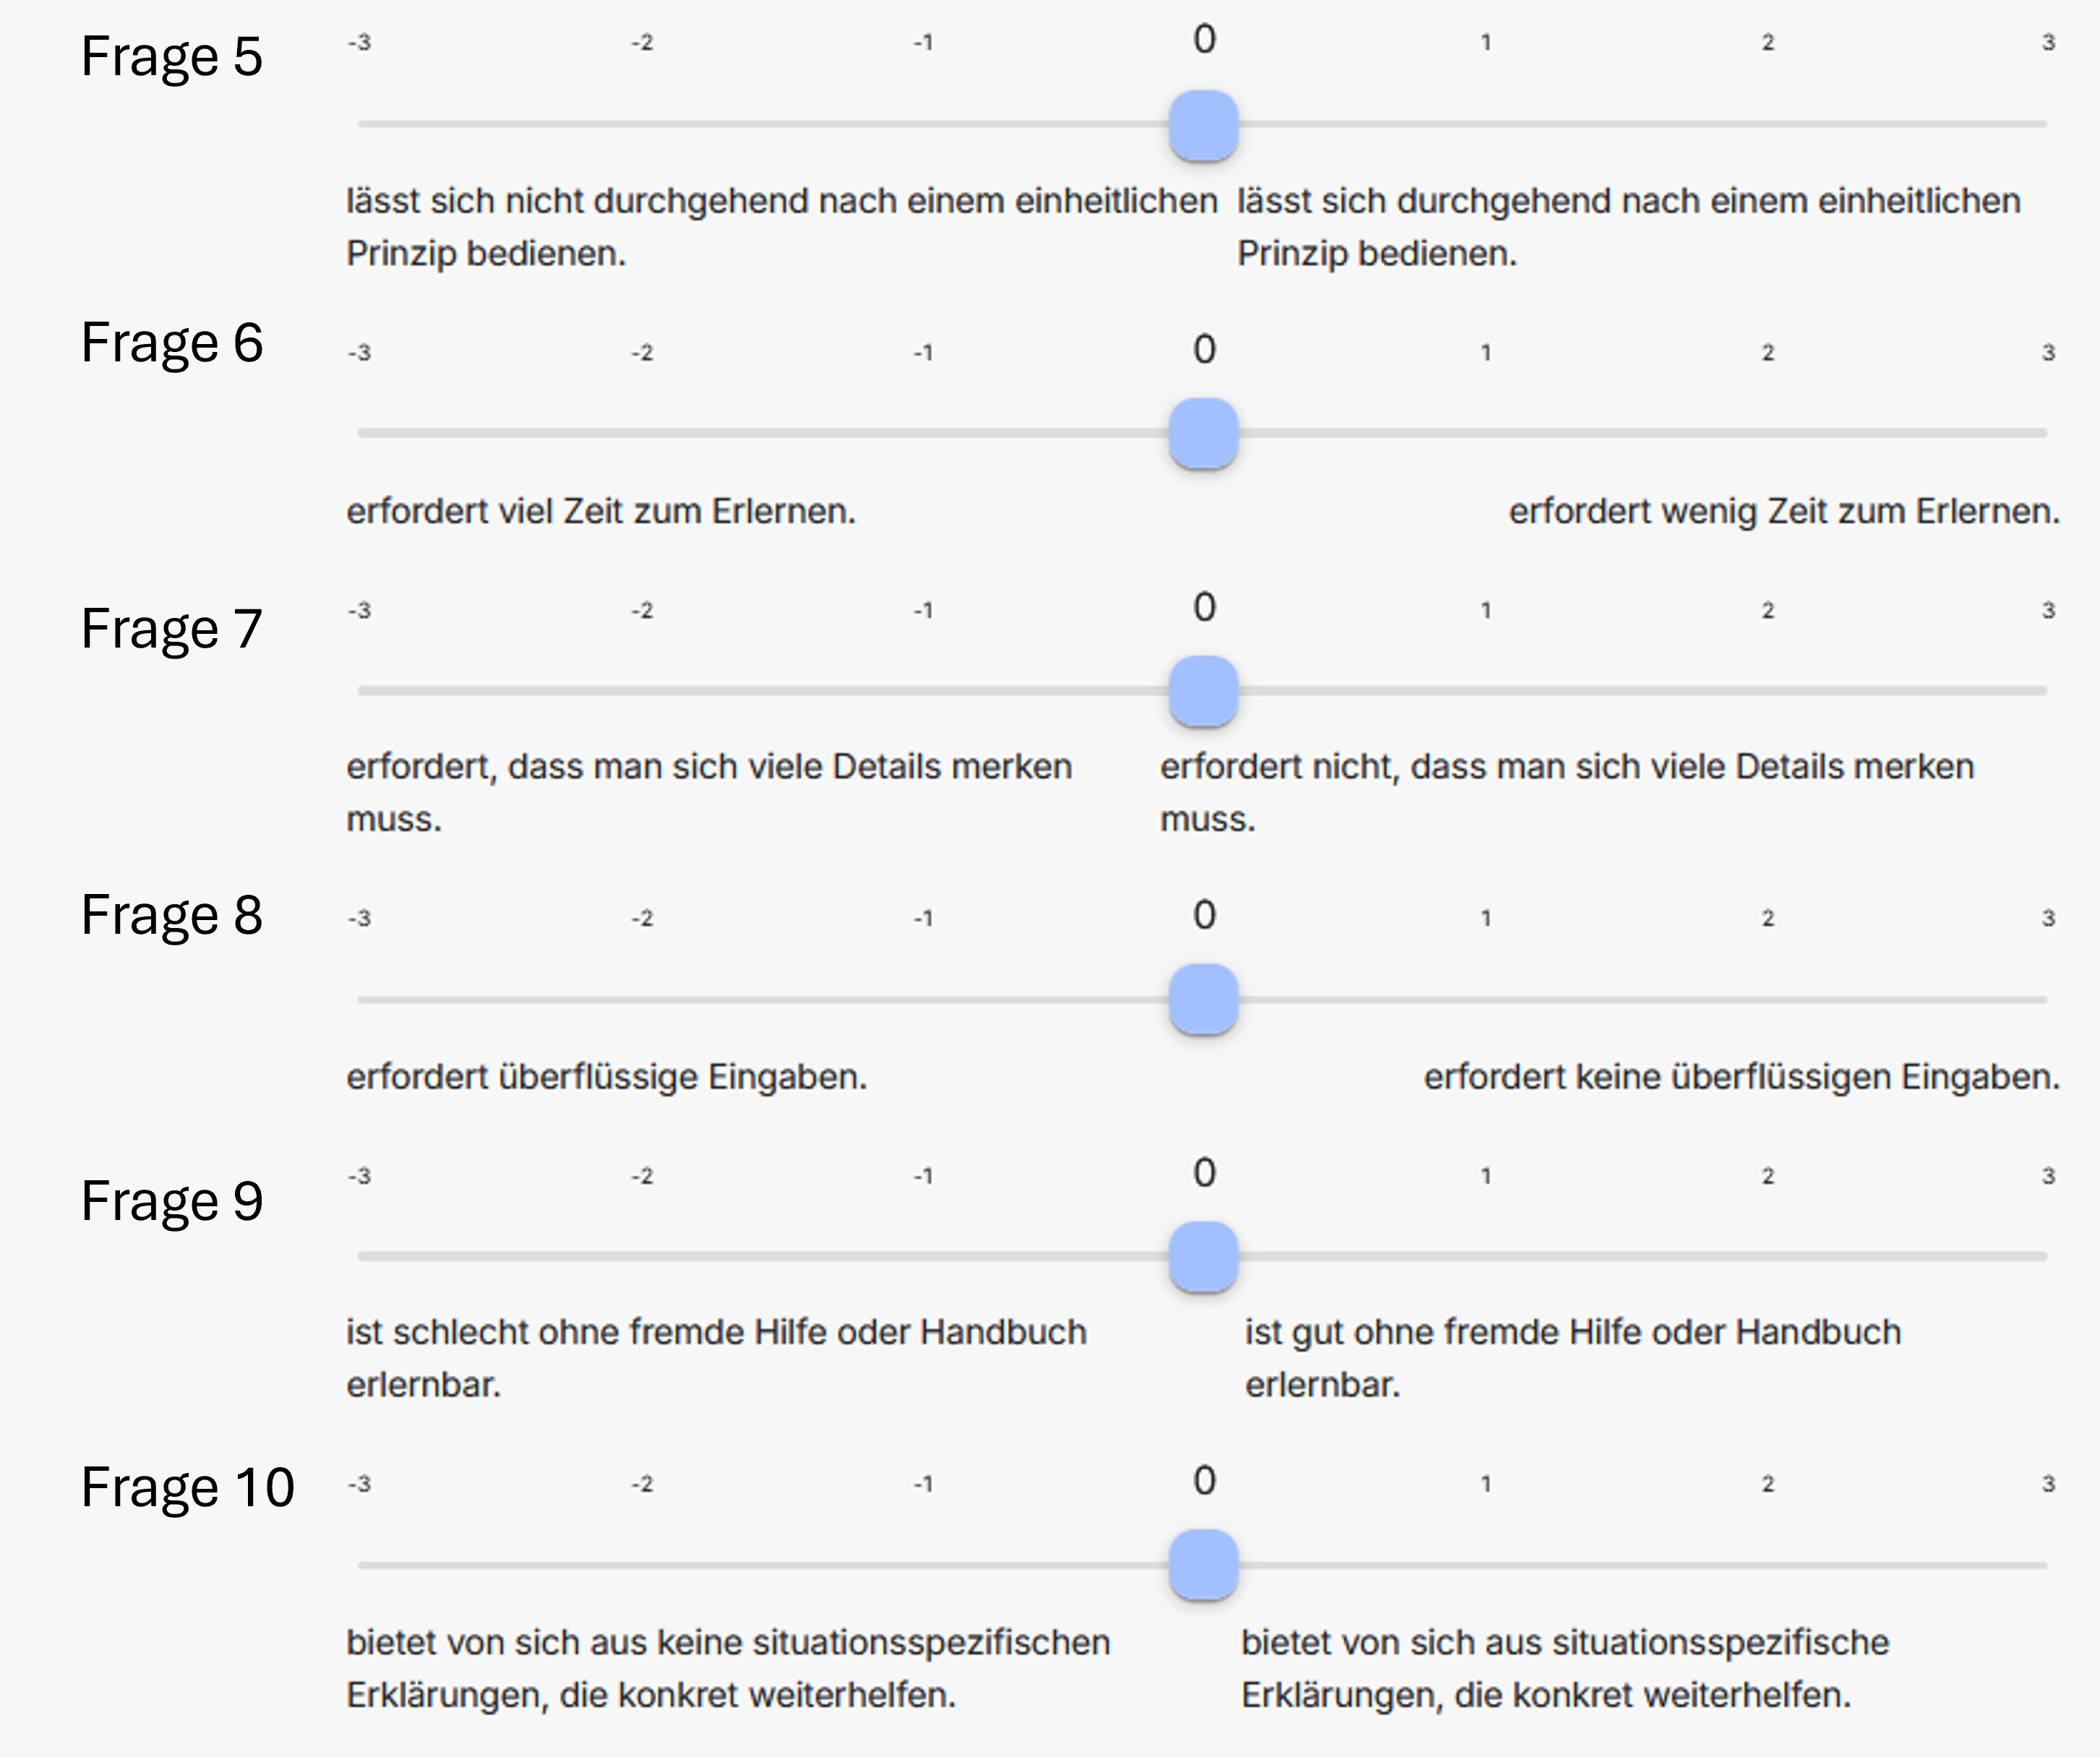
\includegraphics[width=0.85\linewidth]{Anhänge/Survio_Pruemper_2.PNG}
    \caption{gekürzter Fragebogen nach Prümper (Screenshot aus Survio)}
    \label{fig:fragebogen_prümper}
\end{figure}
